\chapter{System considerations}
The following chapter aims to explain some of the considerations we made when we did the preliminary study. 
\section{Platform}
We have worked with several different platforms throughout the courses in our education. A valid choice for platform would be the PSoC 3(5) that we had already worked on. We had been told from other students taking this course that the PSoC was not ideal for sound processing and that the blackfin platform had built in features for this. We had no idea how to use the blackfin so it was a great opportunity to learn to use another platform. 
\subsection{PSoC}
\textbf{Speed:}\\
The PSoC 3 system has a single core running up to 67 MHz. It does not have arithmetic calculation so it might not be ideal for large DSP operations such as cross correlation. \\
\textbf{I/O:}\\
The PSoC has 28 GPIO pins. These can be configured any way you want. The range of the pins is 1.7 V to 5.5 V depending on supply voltage. \\
\textbf{ADC/DMA:}\\
PSoC has a 24-channel DMA which is programmable to access nearly every bus on the board. It has both delta-sigma and sar ADC with up to 20 bits resolution. Sample rate can be up to 192 kHz at 12 bit resolution. \\
\textbf{Memory:}\\
The PSoC has 64 KB of flash memory, 8 KB SRAM and 512-byte cache. This would be enough memory for small signals but would prove difficult if we were to use larger audio signals.\\
\subsection{Blackfin}
\textbf{Speed:}\\
The blackfin processor runs at 600MHz. For every clock it can do two operations (multiplication and/or addition). This effectively means that we can do 1200 million operations per second, if we use the processor 100\% of the time.\\
\textbf{I/O:}\\
The blackfin has an output range of 0 - 0.4 V low to 2.4 - 3.6 high. Input range is -0.3 to 3.6 V. Most of the blackfins I/O is controller by ports. All the phono plugs are connected to the port "Sport0". 
\textbf{ADC \& Audiocodec:}\\
The blackfin has a built-in audiocodec consisting of 4 ADCs and 6 DACs with a resolution of 24 bits. It has a signal to noise ratio of 105dB\footnote{http://www.analog.com/en/audiovideo-products/audio-codecs/ad1836/products/product.html}. There is an example project in the VisualDSP++ environment explaining how to utilize this codec.\\
\textbf{Memory:}\\
Since we do not use much memory we use the L1 cache in the BF533. It is according to the datasheet 32Kbytes big. Since we work with the datatype "short", which is 16 bits, we have enough space for 16K samples.\\
\begin{figure}[hbpt]
\centering
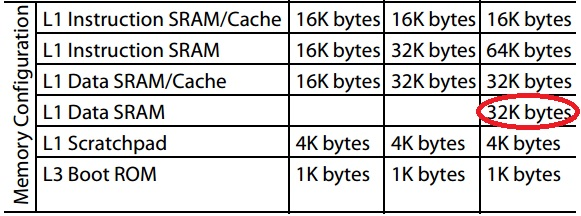
\includegraphics[width=0.5\textwidth]{billeder/memorytable}
\caption[Screen dump from datasheet]{Screen dump from datasheet\footnotemark}
\label{img:mem_table}
\end{figure}
\footnotetext{\url{http://www.analog.com/static/imported-files/data_sheets/ADSP-BF531_BF532_BF533.pdf}}
\subsection{DK8K}
We chose to ignore the DK8K platform as it does not have an Interactive Developer Environment(IDE). This would put a bigger workload on us but would not help us understand how to take advantage of Digital signal processing on embedded units.
\section{Fixed-/FloatingPoint}
\subsection{Floating Point}
Floating point is a way of give approximation of a real value. Usually when working with floating point we have a fixed number of significant digits. A way of presenting a floating point number is "1.2345". Floating point types in c are double and float. The main advantage of floating point is high precision. This comes at a cost of performance and component price.\\
\subsection{Fixed Point}
Fixed point arithmetic is a way to represent a number that has a fixed number of digits before and after the the decimal "." point. Fixed point arithmetic is especially useful for representing fract data types in base 2 or base 10. A way to represent "1.23" in fixed point is "1230". A scaling factor was used. Scaling factors are usually base 2 or base 10. The main advantage of fixed point is performance. This comes at a price of precision. Some embedded microprocessors can not process floating point as it requires a floating point unit(FPU).\\

\section{Technology}
\subsection{Ultrasound}
The first method we discussed was ultrasound. But if we were to choose ultrasound we wouldnt have much data processing since we would just have a transmitter/reciever circuit which has an electrical interface. And wo wouldnt learn much about implementing digital signal processing. Peter also 

\subsection{Laser}
We didnt realy consider laser since we would rather try to play around with sound and measurements of sound. We also figured it would be a lot more complicated for this type of project.

\subsection{Audio}
We went along with hearable sound by suggestion from Peter. Hearable sound is easier to work with since, yes we can hear it, but it is easier to measure and produce. When we record sound we also get a lot of sample which we can process.

\section{Equipment}
\subsection{I/O}
\fixme{If we remember what this was about}
\subsection{Ultrasonic sensor}
We had an ultrasonic sensor of the brand "Ping)))". This didnt really conflict with the concern about using ultrasound since it had a simple electrical interface, but it was not much about digital signal processing but more about timing so we didn't feel it was a good way to go.
\subsection{Speaker/Mic}
If we were to use a speaker combined with a microphone, the first thing we needed was the actual components. We also had to find out how exactly we were to connect these units to the blackfin. The microphone would have to have input biasing as the input channel on microprocessors usually range from 0V to 3.3V or 5V. The speaker would either have to be active or we would be connected to an amplifier. 
